\documentclass{article}[a4paper]
\usepackage[a4paper, total={6in, 9.5in}]{geometry}
\usepackage{charter}
\usepackage{xcolor}
\usepackage{graphicx}
\usepackage{float}
\usepackage{listings}
\usepackage{tabularray}
\usepackage{amsmath}
\usepackage{amssymb}
\usepackage{enumitem}
\usepackage[hidelinks]{hyperref}

\lstset{
  language=Python,
  basicstyle=\ttfamily,
  keywordstyle=\color{blue},
  commentstyle=\color{gray},
  stringstyle=\color{red},
  showstringspaces=false,
  columns=fullflexible,
  breaklines=true
}

\title{
	\huge{\textbf{
		Assignment 01
	}}\\
	\Large{
		Learning from Data, Related Challenges, Linear Models for Regression
	}\\
	\large{\phantom{}}\\
	\large{
		submitted for
	}\\
	\LARGE{
		\textbf{EN3150 - Pattern Recognition}
	}\\
	\large{
		Department of Electronic and Telecommunication Engineering
	}
	\\
	\large{University of Moratuwa}
}

\author{
	\textbf{Udugamasooriya P. H. J.}\\
	220658U % \quad - \quad \href{https://github.com/pulasthi-u/en3160-assignment01}{GitHub}\\
}

\date{12 August 2025}

\allowdisplaybreaks
\setlength{\parindent}{0pt}

\begin{document}

	\maketitle

	\section{Impact of Outliers on Linear Regression}

	\textbf{Question 02}
	We represent the independent variables in a matrix \[
		\mathbf{X} = \begin{pmatrix}
			1		& x_1		\\
			\vdots	& \vdots	\\
			1		& x_n
		\end{pmatrix},
	\] the dependent variables in a vector \[
		\mathbf{y} = \begin{pmatrix}
			y_1 & \cdots & y_n
		\end{pmatrix} ^ \top,
	\] and directly use the result that \[
		\mathbf{w}_\text{OLS}
		=
		\begin{pmatrix} w_0 & w_1 \end{pmatrix} ^ \top
		=
		\underset{\mathbf{w}}{\arg\min}
		\left( \mathbf{y} - \mathbf{X} \mathbf{w} \right)^2
		=
		\left( \mathbf{X}^\top \mathbf{X} \right)^{-1} \mathbf{X}^\top \mathbf{y}.
	\]
	
	This is exactly what we do in code X, and the results obtained from it are as follows:
	\begin{verbatim}
Ordinary Least Squares Weights (w): [ 3.91672727 -3.55727273]
	\end{verbatim}

	Hence, \[
		\mathbf{w}_\text{OLS} = \begin{pmatrix} 3.91672727 \\ -3.55727273 \end{pmatrix},
	\] and the predicted linear model is \[
		y = 3.91672727 - 3.55727273 x.
	\]

	A plot of the given data points against the predicted values is shown in Figure \ref{q1}.

	\begin{figure}[H]
		\centering
		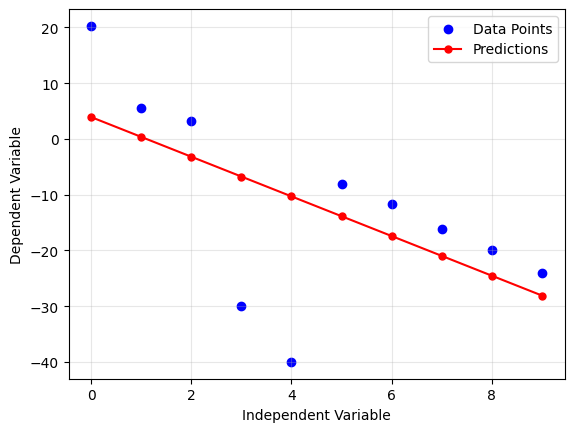
\includegraphics[width=0.8\linewidth]{images/q1.png}
		\caption{abc}
		\label{q1}
	\end{figure}

	\textbf{Question 04} The code in X was used to calculate the loss for each model for each given value
	of $\beta$.
	
	The output of the code was the following:
\begin{verbatim}
Model 1 : [12 -4]
	 Loss for beta = 1      : 0.435416262490386
	 Loss for beta = 1e-06  : 0.9999999998258207
	 Loss for beta = 1000.0 : 0.0002268287498440988
Model 2 : [ 3.91 -3.55]
	 Loss for beta = 1      : 0.9728470518681676
	 Loss for beta = 1e-06  : 0.9999999999999718
	 Loss for beta = 1000.0 : 0.00018824684654645654
\end{verbatim}

	Summarizing these results in a table, we have
	\begin{table}[H]
		\centering
		\begin{tblr}{
			colspec={X[1, c] X[1, c] X[1, c]},
			hlines, vlines,
			width=0.8\textwidth
		}
			$\beta$		& Model 1 Loss	& Model 2 Loss \\
			$1$			& $0.4354$		& $0.9728$ \\
			$10^{-6}$	& $0.9999$		& $1.0000$ \\
			$10^3$		& $0.0002$		& $0.0002$ \\
		\end{tblr}
		\caption{s}
	\end{table}

	\textbf{Question 05} We propose setting $\beta = 1$ to mitigate the impact of outliers.
	\newline

	With very small values of $\beta$, the squared error term starts to dominate, and the loss becomes
	approximately equal to $1$, i.e., \[
		\dfrac{\left(y_i - \hat{y_i}\right)^2}{\left(y_i - \hat{y_i}\right)^2 + \beta^2}
		\approx
		\dfrac{\left( y_i - \hat{y_i} \right)^2}{\left( y_i - \hat{y_i} \right)^2}
		=
		1,
	\] making the result almost independent of the model used, and making it difficult to distinguish
	between several models.
	\newline
	
	% tend to force the squared error term to become very small. In the presence
	% of outliers, a model that closely approximates the behavior of the inliers would produce very large
	% squared errors for the outliers, dominating the loss function. If we try to force the squared errors
	% to be as small as possible then, the model would have to settle somewhere between the inliers and outliers,
	% significantly away from the true model, just so that the error to the outliers is small enough.
	
	Very large values of $\beta$ would cause the loss to be approximately proportional to the squared error and
	very close to $0$, i.e., \[
		\dfrac{\left( y_i - \hat{y_i} \right)^2}{\left( y_i - \hat{y_i} \right)^2 + \beta^2}
		\approx
		\dfrac{\left( y_i - \hat{y_i} \right)^2}{\beta^2}
		\approx
		0,
	\] again making it difficult to distinguish between models. Further, inimizing the loss in this
	case would yield approximately the same result as that of minimizing the mean squared error.
	\newline

	It can be seen from the results above that $\beta = 10^3$ is too large, as the resulting losses from both
	models are both approximately equal, and very small and close to zero, making it difficult to distinguish
	between the two models.
	\newline

	We can also see that $\beta = 10^{-6}$ is too small, as the resulting losses from the models in this 
	case are again both approximately equal but this time close to $1$, leading to the same problem as above.
	\newline

	Hence, $\beta = 1$ is the best choice of the given options, as it has yielded comparable losses for both
	models.
	\newline

	\textbf{Question 06} We will fix $\beta = 1$. The loss for Model 1 then, is $0.4354$, whereas the loss
	for Model 2 is $0.9728$. Clearly, Model 1 has a lower loss and is therefore the better/more suitable model.
	\newline

	\textbf{Question 07} Let us start by rewriting the loss for a single data point as follows: \[
		L\left(y_i, \hat{y_i}, \theta, \beta\right)
		=
		\begin{cases}
			\dfrac{1}{1 + \frac{\beta^2}{\left(y_i - \hat{y_i}\right)^2}},	& y_i \ne \hat{y_i}, \\
			0,																& \text{otherwise}.
		\end{cases}
	\] It is clear then that for all $\hat{y_i}$, the loss is always non-negative and less than $1$, with
	small values of $\left(y_i - \hat{y_i}\right)^2$ resulting in losses close to $0$ and larger values
	resulting in losses close to $1$; and importantly, this property also holds true for outliers.
	\newline

	This has the effect of keeping the loss restricted to a finite range, especially in the presence of outliers,
	in which case a simpler loss such as the squared error would become very large, and not be bounded above.
	\newline
	
	Further, because the loss is always non-negative, the mean loss over all the data points is minimized when
	the loss from each individual data point is as small as possible.
	\newline
	
	Suppose we choose some threshold $E \in (0, 1)$ such that we would like to have \[
		\dfrac{1}{1 + \frac{\beta^2}{\left(y_i - \hat{y_i}\right)^2}} \leq E.
	\] This is equivalent to requiring \[
		\left(y_i - \hat{y_i}\right)^2 \leq \dfrac{E}{1 - E} \cdot \beta^2,
		\quad \text{or} \quad
		\left|y_i - \hat{y_i}\right| \leq \sqrt{\dfrac{E}{1 - E}} \cdot \beta.
	\] Note that this defines an interval of values centered around the actual value $y_i$, that the
	predicted $\hat{y_i}$ might lie within, for which the loss can still be considered "small enough",
	and $\beta$ allows us to control how big or small this interval is. $\beta$ can be chosen
	big enough to include the large distance that the outliers are away from what one might expect their
	true values to be.
	\newline

	Hence, with this modification in place, we prevent the outliers from introducing very large losses, and encourage
	the model to focus more on minimzing the loss due to the inliers, which would contribute more significantly
	to the mean loss, due to the larger number of inliers compared to outliers.
	\newline

	\textbf{Question 08} different loss

	\section{Loss Functions}

	\textbf{Question 01} We calculate the squared error \[
		\text{SE}(\hat{y}_i, y_i) = (\hat{y}_i - y_i)^2
	\] and binary cross entropy \[
		\text{BCE}(\hat{y}_i, y_i) = -y_i \log(\hat{y}_i) - (1 - y_i) \log(1 - \hat{y}_i)
	\] of each predicted value $\hat{y}_i$ against the given corresponding target value $y_i$.
	\begin{table}[H]
		\centering	
		\begin{tblr}{
			colspec={X[1, c] X[1, c] X[1, c] X[1, c]},
			vlines, hlines,
			width=0.8\textwidth
		}
			True Value ($y_i$)	& Predicted Value ($\hat{y_i}$)	& $\text{SE}(\hat{y}_i, y_i)$	& $\text{BCE}(\hat{y}_i, y_i)$ \\
			1 					& 0.005 						& 0.9900 						& 5.2983 \\
			1 					& 0.010 						& 0.9801 						& 4.6052 \\
			1 					& 0.050 						& 0.9025 						& 2.9957 \\
			1 					& 0.100 						& 0.8100 						& 2.3026 \\
			1 					& 0.200 						& 0.6400 						& 1.6094 \\
			1 					& 0.300 						& 0.4900 						& 1.2040 \\
			1 					& 0.400 						& 0.3600 						& 0.9163 \\
			1 					& 0.500 						& 0.2500 						& 0.6931 \\
			1 					& 0.600 						& 0.1600 						& 0.5108 \\
			1 					& 0.700 						& 0.0900 						& 0.3567 \\
			1 					& 0.800 						& 0.0400 						& 0.2231 \\
			1 					& 0.900 						& 0.0100 						& 0.1054 \\
			1 					& 1.000 						& 0.0000 						& 0.0000 \\
								& Mean							& 0.4402		 				& 1.4407
		\end{tblr}
		\caption{Losses for each predicted value}
	\end{table}
	
	A plot of the different losses against the predicted values is shown in Figure \ref{q2}.

	\begin{figure}[H]
		\centering
		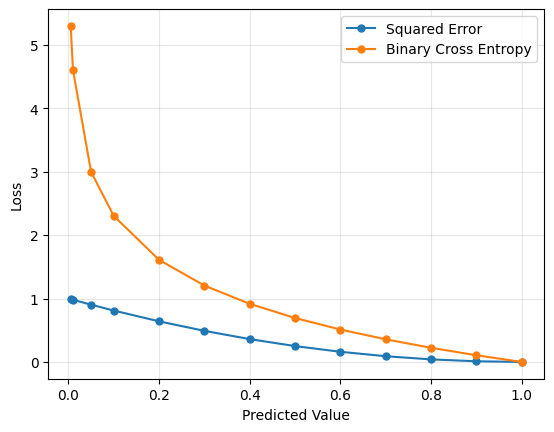
\includegraphics[width=0.7\linewidth]{images/q2.png}
		\caption{abc}
		\label{q2}
	\end{figure}

	\textbf{Question 02}

	\section{Data Pre-Processing}

	\textbf{Question 01} To decide a suitable form of scaling for each feature, we start by visualizing the
	them. The plots in Figure \ref{q3_1} show the distribution of each feature in the dataset.

	\begin{figure}[H]
		\centering
		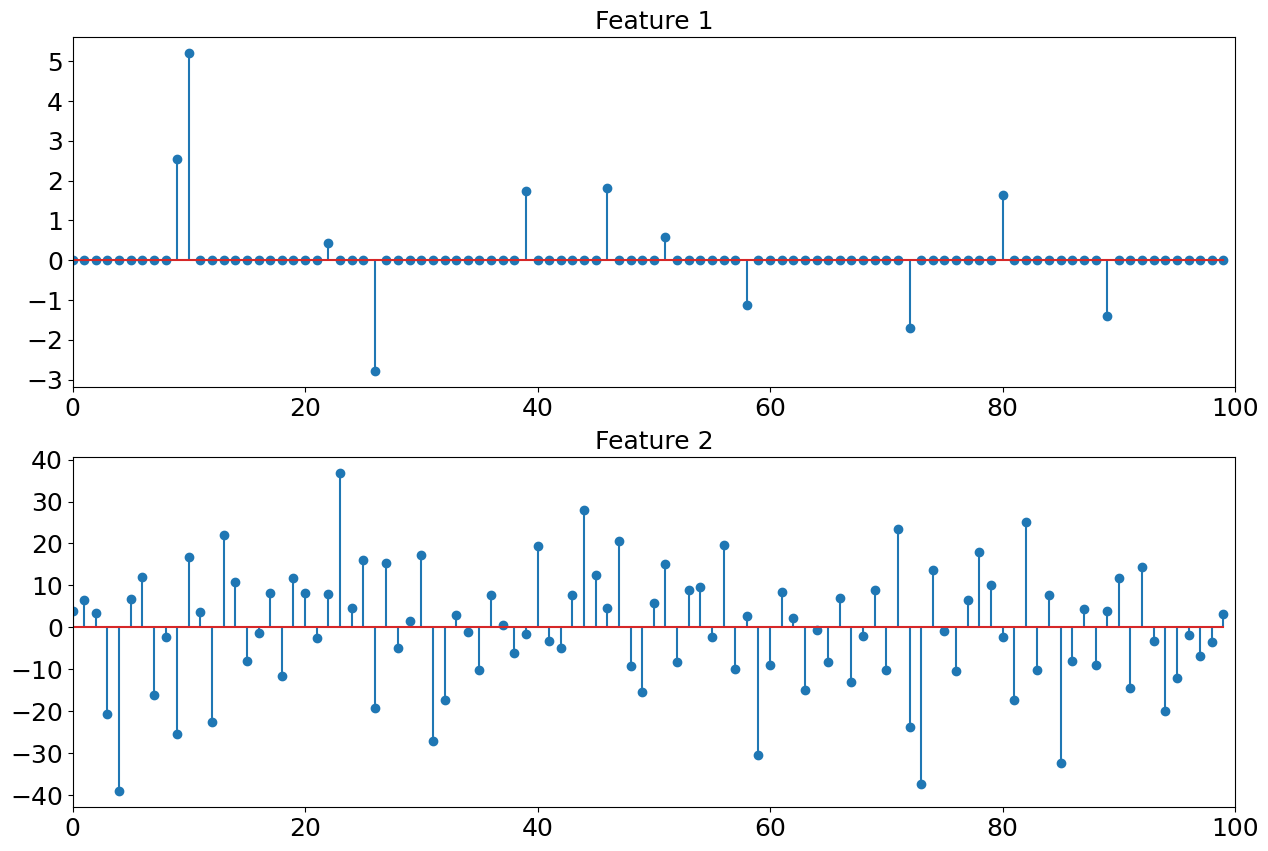
\includegraphics[width=0.7\linewidth]{images/q3_1.png}
		\label{q3_1}
		\caption{abc}
	\end{figure}

	We then run the code in Y to obtain the following summary statistics of each feature:
	\begin{verbatim}
Feature 1
	 Mean 				: 0.06963158220374253
	 Standard Deviation : 0.751690461643816
	 Maximum 			: 5.2
	 Minimum 			: -2.790493210023752
	 Range 				: 7.990493210023752
Feature 2
	 Mean 				: -0.45935709567298505
	 Standard Deviation : 14.351150951654933
	 Maximum 			: 36.752574877667975
	 Minimum 			: -39.11938330852965
	 Range 				: 75.87195818619762
	\end{verbatim}

	Based on the plots above and the above summary statistics, we conclude the following;
	\begin{itemize}
		\item both features have means close to zero
		\item the features vary on different scales, as they have significantly different standard deviations
		\item both features take on both positive and negative values
		\item Feature 1 is sparsely distributed, with most values being equal to 0
	\end{itemize}

	To bring the values of both features to a similar scale, while still preserving the structure and properties of
	each feature, we consider the three following scaling methods;
	\begin{enumerate}
		\item standard scaling,
		\item min-max scaling, and
		\item max-abs scaling.
	\end{enumerate}
	
	We rule out min-max scaling as it would limit both feature values to a range between 0 and 1, affecting the 
	"symmetric" variation among both negative and positive values of both feature values.

	To choose between standard and max-abs scaling, we consider the sparsity of Feature 1. Standard scaling would 
	map the zeros of Feature 1 to non-zero values, resulting in a loss of sparsity, which is a property that
	one would likely want to preserve. Max-abs scaling does not affect sparsity, and maps zeros to zeros. Further, it
	maps to a range between -1 and 1, so negative values map to negative values and positives to positives.

	Hence, we choose max-abs scaling for both feature values. A plot of both feature values after the above scaling
	was applied is shown in Figure \ref{q3_2}. We recalculate the summary statistics for the scaled features too, and
	the results obtained are given below:
	\begin{verbatim}
vab
	\end{verbatim}

\end{document}